%!TEX encoding = UTF-8 Unicode

%\documentclass[14pt]{beamer}
\documentclass{beamer}

\usepackage{listings}
\usepackage{cpp}
% \usepackage{tikz}
\usepackage{pgf-pie}

\usetheme{Copenhagen}
% \usetheme{Boadilla}
% \usecolortheme{beaver}
\setbeamercolor{alerted text}{fg=orange}
\setbeamercolor{background canvas}{bg=white}
\setbeamercolor{block body alerted}{bg=normal text.bg!90!black}
\setbeamercolor{block body}{bg=normal text.bg!90!black}
\setbeamercolor{block body example}{bg=normal text.bg!90!black}
\setbeamercolor{block title alerted}{use={normal text,alerted text},fg=alerted text.fg!75!normal text.fg,bg=normal text.bg!75!black}
\setbeamercolor{block title}{bg=blue}
\setbeamercolor{block title example}{use={normal text,example text},fg=example text.fg!75!normal text.fg,bg=normal text.bg!75!black}
\setbeamercolor{fine separation line}{}
\setbeamercolor{frametitle}{fg=white}
\setbeamercolor{item projected}{fg=white}
\setbeamercolor{normal text}{bg=white,fg=black}
\setbeamercolor{palette sidebar primary}{use=normal text,fg=normal text.fg}
\setbeamercolor{palette sidebar quaternary}{use=structure,fg=structure.fg}
\setbeamercolor{palette sidebar secondary}{use=structure,fg=structure.fg}
\setbeamercolor{palette sidebar tertiary}{use=normal text,fg=normal text.fg}
\setbeamercolor{section in sidebar}{fg=brown}
\setbeamercolor{section in sidebar shaded}{fg=grey}
\setbeamercolor{separation line}{}
\setbeamercolor{sidebar}{bg=red}
\setbeamercolor{sidebar}{parent=palette primary}

\setbeamercolor{structure}{bg=black, fg=white!30!blue!70!green}

\setbeamercolor{subsection in sidebar}{fg=brown}
\setbeamercolor{subsection in sidebar shaded}{fg=grey}
\setbeamercolor{title}{fg=white}
\setbeamercolor{titlelike}{fg=white}

% Szép kék
% \setbeamercolor{structure}{bg=black, fg=white!10!green!40!blue}

\frenchspacing

% Language packages
\usepackage[utf8]{inputenc}
\usepackage[T1]{fontenc}
\usepackage[magyar]{babel}

% AMS
\usepackage{amssymb,amsmath}

% Graphic packages
\usepackage{graphicx}

% Syntax highlighting
\usepackage{listings}

\usepackage{tikz}

\usepackage{hyperref}

% ==============
\begin{document}
% ==============

\title[Alternatív grafikus megjelenítési módok]{Alternatív grafikus megjelenítési módok}
\author[Vécsi Ádám]{\textbf{Vécsi Ádám}}
\institute[]{Miskolci Egyetem}
\date{Miskolci Egyetem, 2018. június 12.}

% --------------------
\frame{\titlepage}

% --------------------
\begin{frame}[fragile]
\frametitle{Művészi szűrők}

Alkalmazási területek
\begin{itemize}
\item Közösségi alkalmazások
\item Webkamera- és mobil alkalmazások
\item Filmek, játékok
\end{itemize}

\bigskip

\begin{center}
\includegraphics[scale=0.25]{kepek/muveszi_szurok/instasnapmess.png}
\end{center}

\end{frame}

% --------------------
\begin{frame}[fragile]
\frametitle{További példák}

\begin{center}
\includegraphics[scale=0.1]{kepek/muveszi_szurok/prismawebcam.jpg}
\end{center}

\begin{center}
\includegraphics[scale=0.1]{kepek/muveszi_szurok/jatekfilm.jpg}
\end{center}

\end{frame}

% --------------------
\begin{frame}[fragile]
\frametitle{Matematikai eszközök}

\textbf{Zajok szűrése, elmosás}

\begin{itemize}
\item Átlagoló szűrő
\item Gauss szűrő
\item Kétoldali szűrő
\item Medián szűrő
$$M =
\begin{bmatrix}
54 &25  &32 \\ 
17 &37  &22 \\ 
11 &23  &45 
\end{bmatrix}$$
Nagyság szerint sorba rendezve ezeket az értékeket, úgy hogy  11, 17, 22, 23, 25, 32, 37, 45, 54 akkor a pixel új intenzitása 25 lesz, mivel az a középső érték a sorban.
\end{itemize}
\end{frame}

% --------------------
\begin{frame}[fragile]
\frametitle{Matematikai eszközök}
\textbf{Élkiemelés}

\begin{itemize}
\item
Sobel éldetektálás
$$
G_x =
\begin{bmatrix}
-1&0  &1 \\ 
-2&0  &2 \\ 
-1&0  &1 
\end{bmatrix},
\qquad
G_y =
\begin{bmatrix}
-1&-2  &-1 \\ 
0&0  &0 \\ 
1&2  &1 
\end{bmatrix}
$$
\item Laplace éldetektálás
\item Canny éldetektálás
\end{itemize}

\end{frame}

% --------------------
\begin{frame}[fragile]
\frametitle{Matematikai eszközök}

\textbf{Szegmentálás}

A célja egyszerűsíteni és/vagy megváltoztatni a kép reprezentációját ezzel könnyebbé téve a kép elemzését.

\begin{itemize}
\item Mean shift algoritmus
\end{itemize}

\bigskip

\textbf{Küszöbölés}

A cél a megfelelő globális és lokális küszöbértékek meghatározása.

\begin{itemize}
\item Izodata algoritmus (Yanni)
\item Otsu algoritmus
\item Niblack algoritmus
\end{itemize}

\end{frame}

% --------------------
\begin{frame}[fragile]
\frametitle{Szűrő algoritmusok}

\textbf{Saját készítésű művészi szűrők}

\begin{itemize}
\item Cartoon-style filter
\item Pencil sketch filter
\item Cartoon filter
\item Aquarelle-style filter
\end{itemize}

\end{frame}

% --------------------
\begin{frame}[fragile]
\frametitle{Cartoon-style filter}
\begin{center}
\textbf{Eredeti kép}
\includegraphics[scale=0.42]{kepek/cartoon_style/image.jpg}
\end{center}
\end{frame}

% --------------------
\begin{frame}[fragile]
\frametitle{Cartoon-style filter}
\begin{center}
\textbf{A Gauss-piramisban kicsinyítés és nagyítás, valamint a kétoldalú szűrő}
\includegraphics[scale=0.42]{kepek/cartoon_style/pyrambilateral.jpg}
\end{center}
\end{frame}

% --------------------
\begin{frame}[fragile]
\frametitle{Cartoon-style filter}
\begin{center}
\textbf{Szürkeárnyalatossá alakított kép, medián szűrő}
\includegraphics[scale=0.42]{kepek/cartoon_style/graymedian.jpg}
\end{center}
\end{frame}

% --------------------
\begin{frame}[fragile]
\frametitle{Cartoon-style filter}
\begin{center}
\textbf{Adaptív küszöbölés az élek kiemelésére}
\includegraphics[scale=0.42]{kepek/cartoon_style/threshold.jpg}
\end{center}
\end{frame}

% --------------------
\begin{frame}[fragile]
\frametitle{Cartoon-style filter}
\begin{center}
\textbf{A szűrökkel és küszöböléssel előállított kép, azaz a Cartoon-Style filter}
\includegraphics[scale=0.42]{kepek/cartoon_style/Cartoon_filter.jpg}
\end{center}
\end{frame}

% --------------------
\begin{frame}[fragile]
\frametitle{Pencil sketch filter}
\begin{center}
\textbf{Eredeti kép}
\includegraphics[scale=0.42]{kepek/pencil_sketch/image.jpg}
\end{center}
\end{frame}

% --------------------
\begin{frame}[fragile]
\frametitle{Pencil sketch filter}
\begin{center}
\textbf{Szürkeárnyalatossá alakított kép, medián szűrő}
\includegraphics[scale=0.42]{kepek/pencil_sketch/mediangray.jpg}
\end{center}
\end{frame}

% --------------------
\begin{frame}[fragile]
\frametitle{Pencil sketch filter}
\begin{center}
\textbf{Gauss szűrő}
\includegraphics[scale=0.42]{kepek/pencil_sketch/gauss.jpg}
\end{center}
\end{frame}

% --------------------
\begin{frame}[fragile]
\frametitle{Pencil sketch filter}
\begin{center}
\textbf{A két szűrő elosztása, kontraszt széthúzás}
\includegraphics[scale=0.42]{kepek/pencil_sketch/contraststrech.jpg}
\end{center}
\end{frame}

% --------------------
\begin{frame}[fragile]
\frametitle{Pencil sketch filter}
\begin{center}
\textbf{Vászon hozzáadása, Pencil sketch filter}
\includegraphics[scale=0.42]{kepek/pencil_sketch/pencil_sketch.jpg}
\end{center}
\end{frame}

% --------------------
\begin{frame}[fragile]
\frametitle{Cartoon filter}
\begin{center}
\includegraphics[scale=0.23]{kepek/cartoon/3_cartoon_filter2.jpg}
\end{center}
\end{frame}


% --------------------
\begin{frame}[fragile]
\frametitle{Aquarelle-style filter}
\begin{center}
\includegraphics[scale=0.23]{kepek/aquarelle_style/4_paint_filter.jpg}
\end{center}
\end{frame}

% --------------------
\begin{frame}[fragile]
\frametitle{Implementáció}

\textbf{OpenCV}

\begin{itemize}
\item Beépített művészi szűrők áttekintése
\begin{itemize}
\item Detail Enhancing filter
\item Stylization
\item Edge Preversing
\item Pencil sketch
\end{itemize}
\begin{center}
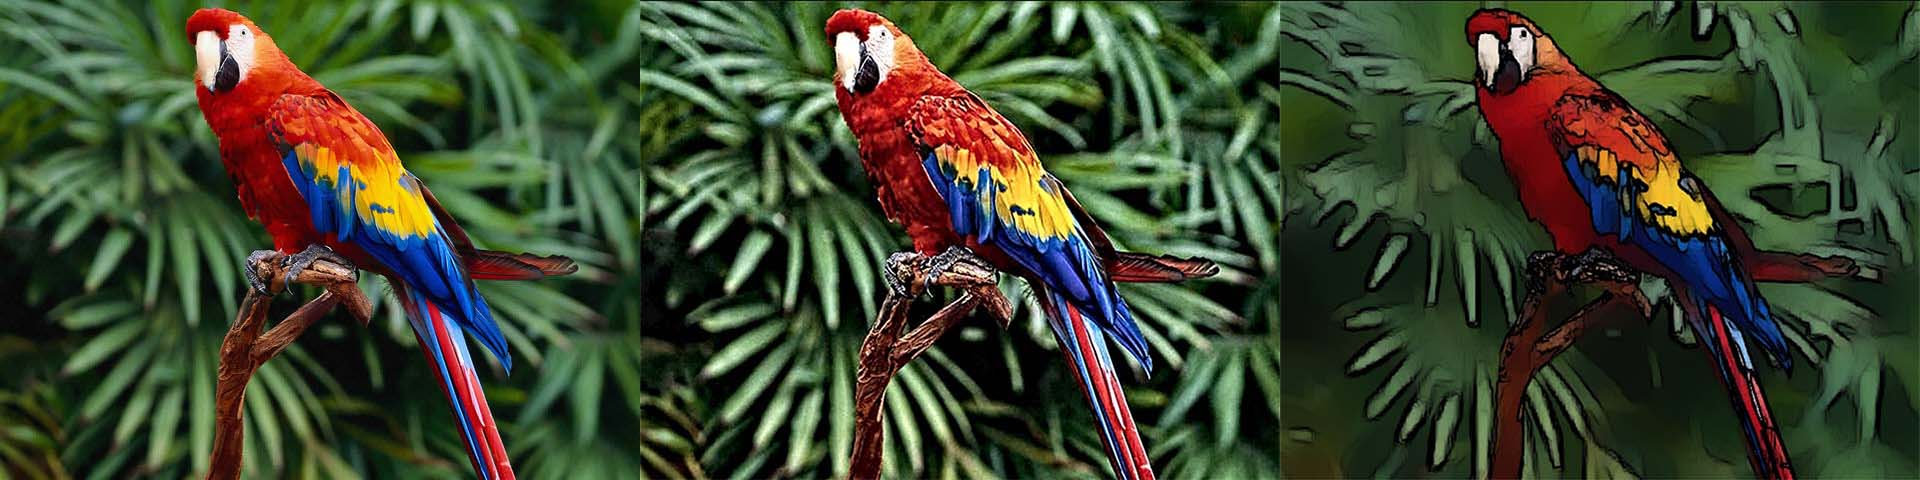
\includegraphics[scale=0.23]{kepek/beepitett_szurok/beepitett_szurok.jpg}
\end{center}
\item Mind a 4 saját szűrőnek külön C++ projekt
\end{itemize}

\medskip

\textbf{Megoldandó feladatok}
\begin{itemize}
\item Képek betöltése, ablak megjelenítése
\end{itemize}

\end{frame}

%\medskip
% --------------------
\begin{frame}[fragile]
\frametitle{Implementáció}

\begin{itemize}
\item Elmosásos szűrők
\end{itemize}

\begin{cpp}
GaussianBlur(source, gauss, ksize, sigmaX, sigmaY);
medianBlur(source, median, kernel_size);
\end{cpp}

\begin{itemize}
\item Élkiemelés
\end{itemize}

\begin{cpp}
Laplacian(source, edges, CV_8U, kernel);
\end{cpp}

\begin{itemize}
\item Szegmentálás
\end{itemize}
\begin{cpp}
pyrMeanShiftFiltering(source, result, sp, sr);
\end{cpp}

\begin{itemize}
\item Küszöbölés
\end{itemize}

\begin{cpp}
threshold(src, res, thr, maxval, THRESH_BINARY_INV);
\end{cpp}


\end{frame}

% --------------------
\begin{frame}[fragile]
\frametitle{Tesztek, eredmények}

\begin{itemize}
\item Elsősorban futási időre vonatkozóan
\item Konfiguráció: MacBook Pro, Intel Core i5, 8GB RAM, Intel Iris
\item Költséges ablaklétrehozási, képbetöltési idők
\item Jelentős számítási idő a konvolúciós műveleteknél
\end{itemize}

\end{frame}

% --------------------
\begin{frame}[fragile]
\frametitle{Cartoon-style filter számítási ideje}
\begin{figure}[h!]
\centering
\resizebox{!}{4.5cm}{
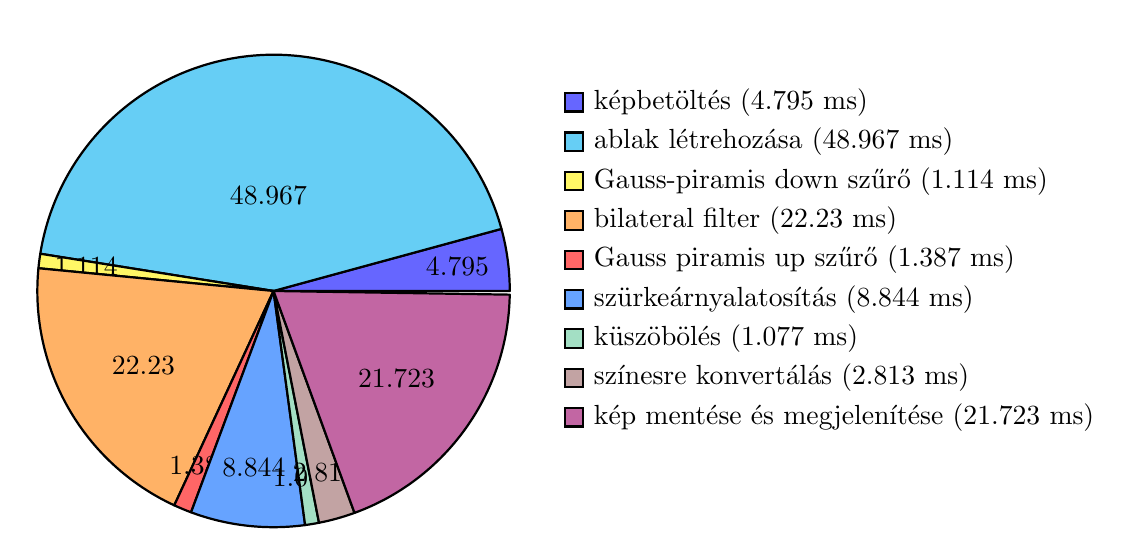
\begin{tikzpicture}
\pie[text=legend, sum=113.229]{
    4.795/képbetöltés (4.795 ms),
    48.967/ablak létrehozása (48.967 ms),
    1.114/Gauss-piramis down szűrő (1.114 ms),
    22.23/bilateral filter (22.23 ms),
    1.387/Gauss piramis up szűrő (1.387 ms),
    8.844/szürkeárnyalatosítás (8.844 ms),
    1.077/küszöbölés (1.077 ms),
    2.813/színesre konvertálás (2.813 ms),
    21.723/kép mentése és megjelenítése (21.723 ms)
}
\end{tikzpicture}
} \\
Cartoon style filter alkalmazásának időigénye (összesen 113.229 ms)
\label{fig:pie1}
\end{figure}
\end{frame}

% --------------------
\begin{frame}[fragile]
\frametitle{Pencil sketch számítási ideje}
\begin{figure}[h!]
\centering
\resizebox{!}{4.5cm}{
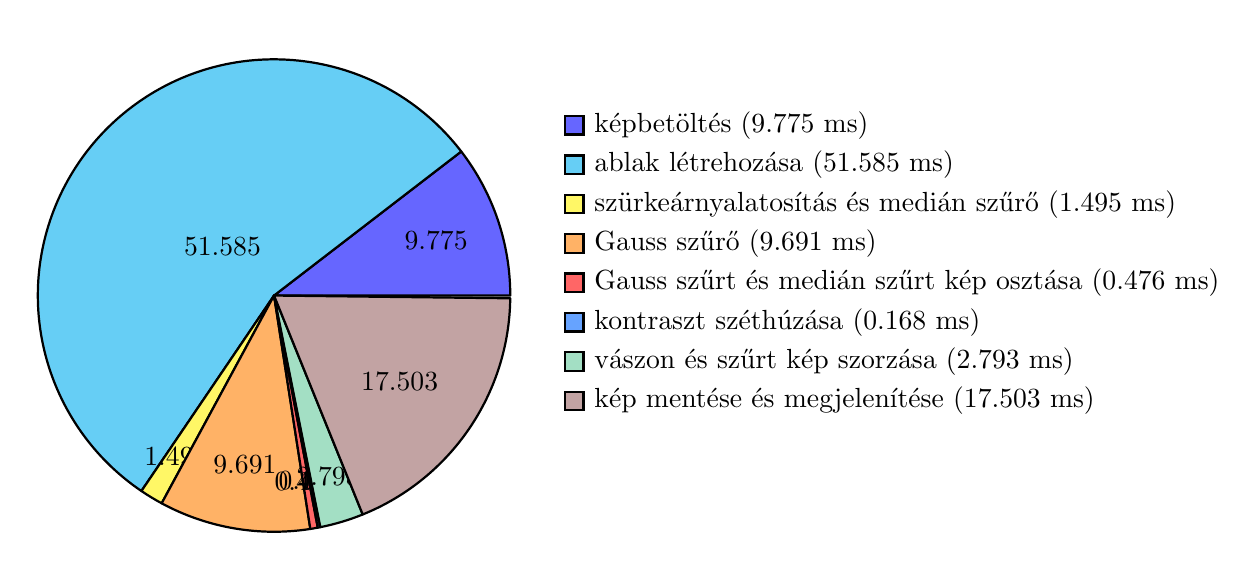
\begin{tikzpicture}
\pie[text=legend, sum=93.661]{
    9.775/képbetöltés (9.775 ms),
    51.585/ablak létrehozása (51.585 ms),
    1.495/szürkeárnyalatosítás és medián szűrő (1.495 ms),
    9.691/Gauss szűrő (9.691 ms),
    0.476/Gauss szűrt és medián szűrt kép osztása (0.476 ms),
    0.168/kontraszt széthúzása (0.168 ms),
    2.793/vászon és szűrt kép szorzása (2.793 ms),
    17.503/kép mentése és megjelenítése (17.503 ms)
}
\end{tikzpicture}
} \\
Pencil sketch filter alkalmazásának időigénye (összesen 93.661 ms)
\label{fig:pie2}
\end{figure}
\end{frame}

% --------------------
\begin{frame}[fragile]
\frametitle{Összegzés}

\begin{itemize}
\item Áttekintettem a képfeldolgozási módszerek matematikai hátterét.
\item Megismerkedtem a \textit{C++}-al és az \textit{OpenCV}-vel.
\item Készítettem 4 saját művészi jellegű szűrőt.
\item Ezeket teszteltem képek és videók esetében is.
\item Lemértem és elemeztem az egyes lépések számítási idejét.
\end{itemize}

\end{frame}

% --------------------
\begin{frame}[fragile]
\frametitle{Hivatkozások}

\begin{thebibliography}{9}

\bibitem[1]{1}
Papari, Giuseppe, Nicolai Petkov, and Patrizio Campisi. Artistic edge and corner enhancing smoothing. IEEE Transactions on Image Processing 16.10 (2007): 2449- 2462.

\bigskip

\bibitem[2]{2}
Kató Zoltán: Digitális képfeldolgozás, egyetemi kurzus, \\
Szegedi Tudományegyetem, \\
\texttt{http://www.inf.u-szeged.hu/ kato/teaching/DigitalisKepfeldolgozasTG}, \\
2014.

\bigskip

\bibitem[3]{3}
Michael Beyeler: How to create a cool cartoon effect with OpenCV and Python, http://www.askaswiss.com/2016/01/ how-to-create-cartoon-effect-opencv-python.html, \\
2016. január 5.

\end{thebibliography}

\end{frame}

% --------------------
\begin{frame}[fragile]
\frametitle{Hivatkozások}

\begin{thebibliography}{9}

\bibitem[4]{4}
Michael Beyeler: How to create a beautiful pencil sketch effect with OpenCV and Python, http://www.askaswiss.com/2016/01/ how-to-create-pencil-sketch-opencv-python.html, \\
2016. január 13.

\bigskip

\bibitem[5]{5}
Shervin Emami: Mastering OpenCV with Practical Computer Vision Projects, Packt Publishing, 2012.

\end{thebibliography}

\end{frame}

% --------------------
\begin{frame}[fragile]
    \frametitle{\ }

\begin{center}
\Large \textbf{Köszönöm szépen a figyelmet!}
\end{center}

\end{frame}


\end{document}